\documentclass[10pt,twocolumn]{article}

\usepackage[T1]{fontenc}
\usepackage{lmodern}
\usepackage[letterpaper,margin=0.72in,columnsep=0.24in]{geometry}
\usepackage{microtype}
\usepackage{booktabs}
\usepackage{tabularx}
\usepackage{siunitx}
\usepackage{enumitem}
\usepackage{graphicx}
\usepackage{xcolor}
\usepackage{tikz}
\usepackage{pgfplots}
\usepackage{natbib}
\usepackage{xurl}
\usepackage[hidelinks]{hyperref}
\usepackage{fancyhdr}
\usepackage{titlesec}

\pgfplotsset{compat=1.18}
\definecolor{paperblue}{HTML}{1D5273}
\definecolor{paperlight}{HTML}{A9C0CF}
\definecolor{papergrid}{HTML}{D8E1E7}
\hypersetup{
  colorlinks=true,
  linkcolor=paperblue,
  citecolor=paperblue,
  urlcolor=paperblue,
  pdftitle={Do Published HumanEval Rankings Survive Local Deployment?},
  pdfauthor={Jaiveer Bassi},
  pdfsubject={Five-model HumanEval ranking reproduction on a consumer GPU}
}

\pagestyle{fancy}
\fancyhf{}
\fancyhead[L]{\scriptsize LOCAL DEPLOYMENT OF CODE MODELS}
\fancyhead[R]{\scriptsize TECHNICAL REPORT \textbar{} 2026}
\fancyfoot[L]{\scriptsize Bassi}
\fancyfoot[R]{\scriptsize \thepage}
\renewcommand{\headrulewidth}{0.35pt}
\renewcommand{\footrulewidth}{0.35pt}
\setlength{\headheight}{13pt}

\titleformat{\section}{\large\bfseries\color{paperblue}}{\thesection.}{0.45em}{}
\titleformat{\subsection}{\normalsize\bfseries\color{paperblue}}{\thesubsection}{0.45em}{}
\titlespacing*{\section}{0pt}{1.1ex plus 0.4ex}{0.6ex}
\titlespacing*{\subsection}{0pt}{0.9ex plus 0.3ex}{0.4ex}
\setlength{\parindent}{0pt}
\setlength{\parskip}{0.45em}
\setlist[itemize]{leftmargin=1.25em,itemsep=0.2em,topsep=0.25em}
\sisetup{detect-all}

\newcommand{\code}[1]{\texttt{#1}}
\newcommand{\pp}{percentage points}

\title{\vspace{-1.5em}\textbf{Do Published HumanEval Rankings Survive Local Deployment?}\\
\large A Five-Model Reproduction on a Consumer GPU}
\author{Jaiveer Bassi\\
\small Independent Researcher, USA\\
\small \href{mailto:jaiveerbassi@yahoo.com}{jaiveerbassi@yahoo.com}}
\date{\small Technical report -- primary experiment, diagnostic ablations, and sampling condition\\Version 1.5, September 19, 2026}

\begin{document}
\maketitle
\thispagestyle{fancy}

\begin{abstract}
Published benchmark tables are often reused as if model rankings were properties of the checkpoints alone. In practice, a score also depends on prompt construction, decoding, stopping, software versions, and execution policy. We tested whether the HumanEval ordering of five open base checkpoints reported together in Table~5 of the Qwen2.5-Coder technical report survives a uniform local deployment condition. Each checkpoint produced one greedy completion for all 164 HumanEval tasks in BF16, at batch size one, on a single NVIDIA RTX~4070. EvalPlus~0.3.1 scored the same completions against HumanEval and HumanEval+ inside a network-isolated container. Four models retained their relative order, but StarCoder2-3B's reported HumanEval score of 31.7\% corresponded to 1.8\% locally, reversing its ordering with Qwen2.5-Coder-0.5B. Kendall's tau-b between published and local HumanEval rankings was 0.8 (task-bootstrap 95\% interval: 0.6 to 0.8). The paired local pass@1 difference for StarCoder2-3B minus Qwen2.5-Coder-0.5B was -21.95~\pp{} (task-bootstrap 95\% interval: -28.66 to -15.85), satisfying the preregistered failure-to-reproduce rule. An unmodified-EvalPlus StarCoder2 control scored 1.2\% (2/164). Post-hoc diagnostics located the cause. EvalPlus~0.3.1 appends a newline to each stripped base-model prompt, a change introduced upstream in August 2024. StarCoder2's tokenizer normally merges that newline with the following indentation; the isolated newline token leads the model to restart the function, which the \code{\textbackslash ndef } stop then truncates to an empty body. Removing only that newline, with every stop retained, raised StarCoder2-3B to 29.9\% (49/164) on HumanEval and 25.6\% (42/164) on HumanEval+, within three tasks of its published values, while the other four checkpoints moved by at most three tasks. Under that condition the published order was recovered exactly (tau-b = 1.0; 95\% interval: 0.8 to 1.0). These results do not show that the published score is erroneous; they show that one prompt byte determines whether this published ordering transfers.
\end{abstract}

\noindent\textbf{Keywords:} code language models; HumanEval; EvalPlus; reproducibility; local inference; functional correctness

\section{Introduction}

HumanEval measures whether generated Python functions satisfy hidden tests and remains a common point of comparison for code language models~\citep{chen2021humaneval}. HumanEval+ strengthens that evaluation with additional automatically generated tests~\citep{liu2023evalplus}. Model reports commonly place scores from several checkpoints in one table, inviting readers to interpret the displayed order as a portable ranking.

That interpretation can be fragile. Functional-correctness results depend on more than weights: prompt templates, stopping strings, generation length, precision, library behavior, and sanitization can all change the executable completion. These choices matter especially for base models, whose training formats and preferred continuation patterns differ.

We reproduce an external and inspectable target: the ordering of five base checkpoints in Table~5 of the Qwen2.5-Coder technical report~\citep{hui2024qwen25coder}. The target contains Qwen2.5-Coder at 0.5B, 1.5B, and 3B parameters, DeepSeek-Coder-1.3B, and StarCoder2-3B. The model families are documented separately by their developers~\citep{hui2024qwen25coder,lozhkov2024starcoder2,guo2024deepseekcoder}. Our question is deliberately narrower than exact score replication: does the published HumanEval ordering survive when all five checkpoints are run through one pinned local stack on a consumer GPU?

The contribution is a completed five-model primary experiment with a predeclared rank endpoint, task-level paired uncertainty, exact checkpoint revisions, raw and sanitized completions, full evaluator outputs, and environment metadata. The principal finding is one statistically resolved rank reversal, followed by a post-hoc diagnosis that attributes it to one documented prompt-construction change in the evaluator. The repository contains the evidence needed to audit that finding at task level~\citep{bassi2026repository}.

\section{Related Work}

HumanEval introduced execution-based functional correctness for 164 handwritten Python synthesis tasks and the pass@$k$ family of estimators~\citep{chen2021humaneval}. EvalPlus subsequently expanded the tests associated with HumanEval and showed that test insufficiency can change both absolute scores and model orderings~\citep{liu2023evalplus}. Our study uses the released HumanEval+ tests but asks a different question: whether a published order transfers across deployment conditions when checkpoint identity and functional tests are held fixed.

The Qwen2.5-Coder report compares several open base models under one table, including all five checkpoints studied here~\citep{hui2024qwen25coder}. StarCoder2 and DeepSeek-Coder are independently documented model families with different training corpora, objectives, and evaluation practices~\citep{lozhkov2024starcoder2,guo2024deepseekcoder}. The EvalPlus leaderboard also lists StarCoder2-3B at 31.7\% HumanEval and 27.4\% HumanEval+ as greedy direct code completion~\citep{evalplus2026leaderboard,evalplus2026setup}. Those values are identical to Table~9 of the StarCoder2 report~\citep{lozhkov2024starcoder2}, and the leaderboard row was added on 29 February 2024, before EvalPlus code generation supported StarCoder2. We therefore treat them as one measurement rather than independent replications. We do not construct a new leaderboard or claim contemporary model coverage. We treat the published table as a concrete external reproduction target and focus on the otherwise underreported inference boundary between weights and executable benchmark candidates.

\section{Research Question and Decision Rule}

The primary question is: \textbf{Does the HumanEval ordering of the five selected checkpoints in Qwen2.5-Coder Table~5 survive the specified local deployment condition?} HumanEval+ is co-reported as a robustness outcome, not substituted for the primary endpoint.

The primary estimand is Kendall's tau-b between the published HumanEval order and the local greedy pass@1 order. We bootstrap tau-b and compare each adjacent pair in the published order using paired resampling over the 164 tasks. Each resample preserves all five model outcomes for a selected task. We use 10,000 bootstrap replicates and fixed analysis seed 2026.

The predeclared decision has three outcomes:

\begin{itemize}
  \item \textbf{Reproduced:} the point ordering is identical, with tau-b equal to 1 and no adjacent published pair reversed locally.
  \item \textbf{Failed to reproduce:} at least one pair is reversed and the paired 95\% bootstrap interval for that pass@1 difference excludes zero in the reversed direction.
  \item \textbf{Inconclusive:} every other outcome, including unresolved ties or reversals whose interval includes zero.
\end{itemize}

This endpoint tests rank transfer, not equality of percentages. Absolute score differences are descriptive because the source paper does not expose every decoding, stopping, and software detail needed to reconstruct Table~5 from the paper alone.

\section{Methods}

\subsection{Models and immutable inputs}

Table~\ref{tab:models} lists the exact base checkpoints and revisions. Revisions were resolved and frozen before aggregate correctness results were inspected.

\begin{table*}[t]
\centering
\caption{Frozen model inputs. Full identifiers also appear in machine-readable protocol metadata.}
\label{tab:models}
\small
\begin{tabularx}{\textwidth}{@{}l l >{\ttfamily\scriptsize}X@{}}
\toprule
Model & Hugging Face checkpoint & \normalfont Revision \\
\midrule
Qwen2.5-Coder-0.5B & Qwen/Qwen2.5-Coder-0.5B & 8123ea2e9354afb7ffcc6c8641d1b2f5ecf18301 \\
StarCoder2-3B & bigcode/starcoder2-3b & 733247c55e3f73af49ce8e9c7949bf14af205928 \\
DeepSeek-Coder-1.3B & deepseek-ai/deepseek-coder-1.3b-base & c919139c3a9b4070729c8b2cca4847ab29ca8d94 \\
Qwen2.5-Coder-1.5B & Qwen/Qwen2.5-Coder-1.5B & df3ce67c0e24480f20468b6ef2894622d69eb73b \\
Qwen2.5-Coder-3B & Qwen/Qwen2.5-Coder-3B & 09d9bc5d376b0cfa0100a0694ea7de7232525803 \\
\bottomrule
\end{tabularx}
\end{table*}

\subsection{Generation condition}

All five models used the EvalPlus base-model HumanEval prompt, with base mode forced even when a tokenizer exposed a chat template. Generation was greedy with one completion per task, a maximum of 512 new tokens, batch size one, and BF16 weights. The models ran sequentially on one NVIDIA GeForce RTX~4070 with 12,282~MiB dedicated memory in WSL Ubuntu on Windows. The generation environment used PyTorch~2.8.0+cu128 and Transformers~4.57.6. No latency or throughput conclusion is drawn from the correctness run.

The primary design uses no repeated random seeds. Conditional on the frozen inputs and software stack, greedy decoding is deterministic; repeated identical runs would measure system nondeterminism rather than sampling variance. The separately specified 20-sample sensitivity condition is reported as a secondary result in Section~\ref{sec:sampling}; it does not enter the primary endpoint.

\subsection{Functional evaluation and execution safety}

The same completions were evaluated on all 164 HumanEval tasks and the corresponding HumanEval+~v0.1.10 tests. We pinned EvalPlus~0.3.1 at commit \code{e5d0ed0bab96280b60b637ec7f15b5e4841b0cb2}. Generated Python was executed only in a disposable Linux container with networking disabled, credentials absent, capabilities dropped, and no writable host mount beyond the result exchange directory.

The official Docker image tagged v0.3.1 exposed a development package version during verification. We therefore derived the evaluator from the official immutable base-image digest, force-installed released \code{evalplus==0.3.1}, asserted the installed version at build time, and recorded the derived image identifier.

\subsection{Harness equivalence checks}

Two changes addressed avoidable generation overhead without changing the declared stopping predicate. First, the upstream batch-one stop criterion decoded the same completion once for each stop string after every token. The wrapper decodes once and checks all stop strings; a pinned one-task comparison required byte-identical raw and sanitized outputs before the full run. Second, EvalPlus left a wrapped Transformers stopping method installed after each task, causing criteria to accumulate. A \code{finally} block restores the original method after generation. We subsequently repeated HumanEval/0 and HumanEval/1 through unmodified EvalPlus for all five checkpoints. Raw and sanitized records were byte-identical to the retained primary records for every model and task. Machine-readable hashes for both checks are included in the repository.

The provider's mutable stop list could also acquire duplicate strings when models were constructed sequentially. The runner removes only exact duplicates while preserving first occurrence and order, leaving the logical \code{any(stop in decoded)} predicate unchanged.

\subsection{Analysis}

Pass@1 is the proportion of 164 tasks for which the single completion passed. At one completion per task this is a direct proportion, not the multi-sample estimator introduced with HumanEval~\citep{chen2021humaneval}. Bootstrap intervals are computed on paired task outcomes. The analysis program rejects missing, duplicate, non-Boolean, or mismatched task records before aggregation.

\section{Results}

Table~\ref{tab:results} reports all primary measurements. Exact counts are included to avoid false precision.

\begin{table*}[t]
\centering
\caption{Qwen2.5-Coder Table~5, EvalPlus leaderboard, and local primary pass@1. HE denotes HumanEval; HE+ denotes HumanEval+. Dashes indicate models absent from the current EvalPlus result data.}
\label{tab:results}
\scriptsize
\begin{tabular}{@{}lrrrrrr@{}}
\toprule
Model & Qwen HE & EvalPlus HE & Local HE & Qwen HE+ & EvalPlus HE+ & Local HE+ \\
\midrule
Qwen2.5-Coder-0.5B & 28.0\% & --- & 23.8\% (39/164) & 23.8\% & --- & 20.1\% (33/164) \\
StarCoder2-3B & 31.7\% & 31.7\% & 1.8\% (3/164) & 27.4\% & 27.4\% & 1.8\% (3/164) \\
DeepSeek-Coder-1.3B & 34.8\% & 28.7\% & 34.1\% (56/164) & 26.8\% & 25.6\% & 28.7\% (47/164) \\
Qwen2.5-Coder-1.5B & 43.9\% & --- & 39.0\% (64/164) & 36.6\% & --- & 34.1\% (56/164) \\
Qwen2.5-Coder-3B & 52.4\% & --- & 52.4\% (86/164) & 42.7\% & --- & 42.7\% (70/164) \\
\bottomrule
\end{tabular}
\end{table*}

The StarCoder2 discrepancy is not confined to the Qwen comparison table. The EvalPlus leaderboard reports the same 31.7\% HumanEval and 27.4\% HumanEval+ values for greedy direct completion~\citep{evalplus2026leaderboard,evalplus2026setup}. Those values match the StarCoder2 report's own Table~9~\citep{lozhkov2024starcoder2}, so all three published sources trace to one measurement. Our unmodified-EvalPlus result of 1.2\% nevertheless conflicts with that measurement under the same evaluator family and nominal mode, which requires a pipeline-level explanation (Section~\ref{sec:diagnostic}).

The published HumanEval order from low to high was Qwen2.5-Coder-0.5B, StarCoder2-3B, DeepSeek-Coder-1.3B, Qwen2.5-Coder-1.5B, and Qwen2.5-Coder-3B. Locally, StarCoder2-3B moved below Qwen2.5-Coder-0.5B; the other four positions retained their relative order. Kendall's tau-b was 0.8, with a paired task-bootstrap 95\% interval of [0.6, 0.8].

For the reversed adjacent pair, the local difference for StarCoder2-3B minus Qwen2.5-Coder-0.5B was -21.95~\pp{}, with paired-bootstrap 95\% interval [-28.66, -15.85]. The interval excludes zero in the reversed direction. The primary decision is therefore \textbf{failed to reproduce}.

The other adjacent local HumanEval differences, in published low-to-high order, were: DeepSeek-Coder-1.3B minus StarCoder2-3B, +32.32 points [25.61, 39.63]; Qwen2.5-Coder-1.5B minus DeepSeek-Coder-1.3B, +4.88 points [-2.44, 12.20]; and Qwen2.5-Coder-3B minus Qwen2.5-Coder-1.5B, +13.41 points [5.49, 21.34]. These intervals are descriptive and do not alter the predeclared decision once a resolved reversal is present.

\begin{figure*}[t]
\centering
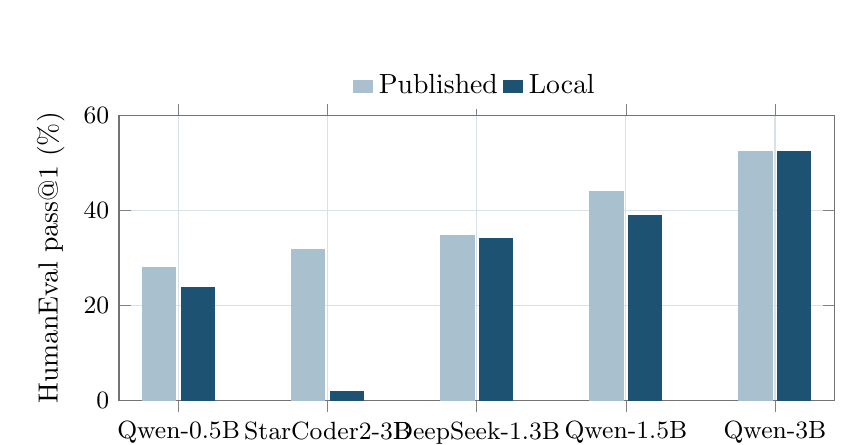
\begin{tikzpicture}
\begin{axis}[
  width=0.88\textwidth,
  height=5.2cm,
  ybar,
  bar width=12pt,
  ymin=0,
  ymax=60,
  ylabel={HumanEval pass@1 (\%)},
  symbolic x coords={Qwen-0.5B,StarCoder2-3B,DeepSeek-1.3B,Qwen-1.5B,Qwen-3B},
  xtick=data,
  x tick label style={font=\small},
  y tick label style={font=\small},
  legend style={at={(0.5,1.02)},anchor=south,legend columns=2,draw=none},
  legend image code/.code={\draw[#1] (0cm,-0.08cm) rectangle (0.24cm,0.08cm);},
  grid=major,
  grid style={draw=papergrid},
  axis line style={draw=black!55},
]
\addplot[fill=paperlight,draw=paperlight] coordinates {
  (Qwen-0.5B,28.0) (StarCoder2-3B,31.7) (DeepSeek-1.3B,34.8)
  (Qwen-1.5B,43.9) (Qwen-3B,52.4)
};
\addplot[fill=paperblue,draw=paperblue] coordinates {
  (Qwen-0.5B,23.8) (StarCoder2-3B,1.8) (DeepSeek-1.3B,34.1)
  (Qwen-1.5B,39.0) (Qwen-3B,52.4)
};
\legend{Published,Local}
\end{axis}
\end{tikzpicture}
\caption{Published and local HumanEval pass@1. The StarCoder2-3B divergence determines the rank-reproduction outcome.}
\label{fig:results}
\end{figure*}

HumanEval+ preserved the same local order. Qwen2.5-Coder-3B matched the displayed published percentage to rounding on both benchmarks; DeepSeek-Coder-1.3B was 1.9 points higher locally on HumanEval+; and the remaining Qwen checkpoints were 2.5 to 4.9 points lower. StarCoder2-3B was the clear outlier, 29.9 points below the displayed HumanEval score and 25.6 points below the displayed HumanEval+ score.

\section{Diagnostic Analysis}
\label{sec:diagnostic}

The StarCoder2-3B result warranted a targeted diagnostic because its absolute difference was much larger than those of the other models. Using the same pinned weights, BF16 precision, and eager Transformers path, the checkpoint generated ordinary Python for the short prompt shown in its model card~\citep{bigcode2024starcoder2card}. We first checked for a decoding error. EvalPlus's Hugging Face provider decodes only tokens generated after the input; the retained raw JSONL begins with the HumanEval prompt because the code-generation layer deliberately serializes \code{prompt + implementation}. The apparent prompt echo in the artifact is therefore not evidence that the provider decoded the full input sequence.

The generated suffix for HumanEval/0 instead begins by repeating the complete function signature and docstring. EvalPlus~0.3.1 registers the exact text \code{\textbackslash ndef } as a generation stop for direct HumanEval completion and then truncates at that boundary. Under the standard stop list, the repeated definition is removed and the candidate contains no body. This mechanism is directly visible in the retained stock and ablation records.

We also reran all 164 StarCoder2 tasks through the unmodified EvalPlus~0.3.1 Hugging Face generation path under the same pinned revision, precision, prompt, decoding, attention, and token limit. Hardened evaluation yielded 2/164 (1.2\%) on both HumanEval and HumanEval+, compared with 3/164 (1.8\%) for the optimized wrapper. The stock run passed HumanEval/49 and HumanEval/53; the primary run additionally passed HumanEval/50. Thus the wrapper changes do not account for the low StarCoder2 score or the rank reversal. Two-task stock checks for every model were also byte-identical to their retained primary raw and sanitized records.

We then ran a clearly labeled post-hoc secondary ablation that removed only \code{\textbackslash ndef } from the stop list. The checkpoint, revision, base prompt, BF16 precision, greedy decoding, batch size, 512-token cap, sanitizer, dataset, and evaluator were unchanged. To avoid the stock provider's accumulating-hook overhead, the full run used the primary decode-once and hook-restoration implementation; its first 20 raw and sanitized records were byte-identical to a separately retained stock-ablation prefix. Hardened evaluation produced 17/164 (10.4\%) on HumanEval and 15/164 (9.1\%) on HumanEval+.

\begin{table}[t]
\centering
\caption{StarCoder2-3B controls and post-hoc ablations. Each ablation changes one factor from the stock condition.}
\label{tab:ablation}
\scriptsize
\begin{tabularx}{\columnwidth}{@{}Xrr@{}}
\toprule
Condition & HE & HE+ \\
\midrule
Primary, standard stops & 1.8\% (3/164) & 1.8\% (3/164) \\
Stock EvalPlus, standard stops & 1.2\% (2/164) & 1.2\% (2/164) \\
Without \code{\textbackslash ndef } stop & 10.4\% (17/164) & 9.1\% (15/164) \\
Without trailing prompt newline & 29.9\% (49/164) & 25.6\% (42/164) \\
Published (StarCoder2 Table~9) & 31.7\% & 27.4\% \\
\bottomrule
\end{tabularx}
\end{table}

Removing the stop recovered 9.15~\pp{} on HumanEval and 7.93~\pp{} on HumanEval+ relative to the stock control, but gaps of 21.3 and 18.3 points to the published values remained. The stop was where the damage became visible, not why the model restarted the function.

\subsection{Trailing prompt newline}

EvalPlus~0.3.1 passes \code{task["prompt"].strip() + "\textbackslash n"} to direct-completion models. Its history shows that this boundary has changed: a commit on 17 March 2024 titled ``fix: starcoder l2r inference'' stripped the prompt, and a commit on 3 August 2024 re-appended the newline~\citep{evalplus2026setup}. Both followed the StarCoder2 report. In StarCoder2's tokenizer, the newline after a closing docstring is normally merged with the following blank lines and indentation into one token. A prompt ending in an isolated newline token places the model at a boundary it rarely sees inside a function, and at HumanEval/0 it begins a new top-level definition.

A second post-hoc ablation retained every stop text and changed only the model input, omitting that final newline. The stored candidate remained \code{prompt + completion}, so sanitization and evaluation were unchanged. Because a prompt change could affect every model, we ran it for all five checkpoints and applied the preregistered analysis code descriptively. Table~\ref{tab:newline} reports the hardened evaluation.

\begin{table}[t]
\centering
\caption{Passes out of 164 for all five checkpoints in the primary condition and without the trailing prompt newline.}
\label{tab:newline}
\scriptsize
\begin{tabularx}{\columnwidth}{@{}Xrrrr@{}}
\toprule
 & \multicolumn{2}{c}{Primary} & \multicolumn{2}{c}{No newline} \\
Model & HE & HE+ & HE & HE+ \\
\midrule
Qwen2.5-Coder-0.5B & 39 & 33 & 37 & 31 \\
StarCoder2-3B & 3 & 3 & 49 & 42 \\
DeepSeek-Coder-1.3B & 56 & 47 & 54 & 46 \\
Qwen2.5-Coder-1.5B & 64 & 56 & 67 & 56 \\
Qwen2.5-Coder-3B & 86 & 70 & 85 & 71 \\
\bottomrule
\end{tabularx}
\end{table}

StarCoder2-3B rose from 2--3 passes to 49/164 (29.9\%) on HumanEval and 42/164 (25.6\%) on HumanEval+, three tasks below both published values. The other checkpoints changed by at most three tasks. The local order matched the published order exactly: Kendall's tau-b was 1.0, with a paired task-bootstrap 95\% interval of [0.8, 1.0]. Adjacent differences in published order were +7.32 points [1.83, 12.80] for StarCoder2-3B minus Qwen2.5-Coder-0.5B, +3.05 [-2.44, 8.54] for DeepSeek-Coder-1.3B minus StarCoder2-3B, +7.93 [0.61, 15.24] for Qwen2.5-Coder-1.5B minus DeepSeek-Coder-1.3B, and +10.98 [3.66, 18.29] for Qwen2.5-Coder-3B minus Qwen2.5-Coder-1.5B. Applied to these outcomes, the preregistered rule would return \emph{reproduced}. Because the condition was chosen after the primary result, it does not replace the primary decision; it identifies the documented evaluator change on which that decision depends.

\section{Stochastic Sensitivity}
\label{sec:sampling}

The preregistered secondary condition draws 20 samples per task at temperature 0.2 with top-p 0.95, seed 11, BF16 weights, and the same prompt, stop texts, 512-token cap, and evaluator as the primary run. It covers the three resource-matched checkpoints named in the plan. We add one post-hoc run: StarCoder2-3B without the trailing prompt newline, so the diagnosis of Section~\ref{sec:diagnostic} can be checked outside greedy decoding. All four runs completed without interruption, and pass@$k$ uses the unbiased estimator~\citep{chen2021humaneval} with paired task-bootstrap intervals.

\begin{table}[t]
\centering
\caption{Twenty-sample pass@$k$ on HumanEval with paired task-bootstrap 95\% intervals, beside the corresponding greedy pass@1.}
\label{tab:sampling}
\scriptsize
\begin{tabularx}{\columnwidth}{@{}Xrrr@{}}
\toprule
Condition & pass@1 & pass@5 & Greedy \\
\midrule
Qwen2.5-Coder-1.5B & 37.6 [31.2, 44.1] & 50.8 [43.8, 57.8] & 39.0 \\
DeepSeek-Coder-1.3B & 32.2 [25.9, 38.7] & 41.3 [34.2, 48.6] & 34.1 \\
StarCoder2-3B, stock & 2.3 [0.9, 4.2] & 5.6 [2.8, 8.7] & 1.8 \\
StarCoder2-3B, no newline & 29.8 [23.7, 36.2] & 40.4 [33.4, 47.4] & 29.9 \\
\bottomrule
\end{tabularx}
\end{table}

Table~\ref{tab:sampling} shows that sampling pass@1 falls within about two points of greedy pass@1 in every condition, so the primary greedy measurements are not unusual draws. StarCoder2-3B remains at 2.3\% under the stock prompt with 20 samples per task; its primary result is therefore not an artifact of greedy decoding, and the trailing-newline condition recovers it here as it does under greedy decoding. HumanEval+ pass@1 follows the same pattern at 31.5\%, 27.8\%, 2.3\%, and 26.1\%.

Seeds 23 and 37 were not run. The plan triggers them only on a rank reversal or an adjacent pair below five \pp{}; the seed-11 ordering is preserved and the closest adjacent pair differs by 5.37~\pp{}. That margin is narrow, so the untriggered condition should not be read as a wide separation.

DeepSeek-Coder-1.3B generated at batch size 2 rather than 20 because its multi-head key/value cache for 20 concurrent sequences exhausts the 12\,GB GPU, after which the driver spills into host memory. Batch size affects throughput only; sample count, temperature, top-p, prompt, stop texts, and token cap are identical across conditions.

\subsection{Prompt and quantization ablations}

The plan assigns two further single-factor conditions to Qwen2.5-Coder-1.5B at seed 11, holding the reference sampling settings fixed. The first stops forcing the base prompt: the checkpoint ships a chat template, so EvalPlus builds its instruction-style prompt using its own default instruction and response prefixes. The second loads bitsandbytes 8-bit weights in place of BF16. Each run verifies at load time that the intended path was taken, so a silent fallback to the reference condition fails rather than producing a misleading number. Differences are paired: the 164 tasks are resampled with each task's two per-task pass@1 estimates kept together.

\begin{table}[t]
\centering
\caption{Qwen2.5-Coder-1.5B single-factor ablations against the 20-sample reference condition, with paired task-bootstrap 95\% intervals on the pass@1 difference.}
\label{tab:qwen-ablations}
\scriptsize
\begin{tabularx}{\columnwidth}{@{}Xrrr@{}}
\toprule
Condition & pass@1 & pass@5 & Paired difference \\
\midrule
Reference (BF16, base prompt) & 37.6 & 50.8 & --- \\
Chat-template prompt & 48.6 & 66.5 & $+11.07$ [4.39, 17.74] \\
8-bit weights & 24.4 & 34.4 & $-13.17$ [$-17.90$, $-8.66$] \\
\bottomrule
\end{tabularx}
\end{table}

Table~\ref{tab:qwen-ablations} shows that both intervals exclude zero. HumanEval+ moves in the same directions, to 43.7\% for the chat prompt ($+12.23$ [5.64, 18.96]) and 23.2\% for 8-bit ($-8.23$ [$-12.29$, $-4.24$]). These conditions cover one checkpoint and do not bear on the primary decision, but they bound how much ordinary deployment choices matter: a prompt-mode change and an 8-bit load move one checkpoint by roughly 11 and 13~\pp{}, which exceeds most adjacent gaps in the published table. The same reasoning that makes the trailing-newline result a pipeline property applies here.

\section{Threats to Validity}

\textbf{Target specification.} The published percentages and model identities are available in Qwen2.5-Coder Table~5, but the report does not specify every generation and post-processing detail for that table. The current public evaluation-code link associated with the report is not, by itself, an immutable reconstruction of the historical run. Our experiment therefore tests transfer to a disclosed condition, not faithful rerun of an undisclosed condition.

\textbf{Single deployment stack.} The primary run used one GPU, one precision, one inference library version, and one evaluator release, and does not estimate variation across hardware, kernels, or libraries; it also does not support CPU performance claims. The prompt and 8-bit ablations of Section~\ref{sec:sampling} probe two of those axes on a single checkpoint and are not a general characterization of prompt mode or quantization.

\textbf{One greedy completion.} The primary endpoint measures deterministic greedy pass@1. The secondary 20-sample condition in Section~\ref{sec:sampling} characterizes sampling at one temperature and one seed for three checkpoints; it does not cover the remaining models, other temperatures, or repeated seeds. The task bootstrap quantifies uncertainty across the finite task set, not across sampler seeds.

\textbf{Benchmark scope.} HumanEval contains 164 Python tasks. HumanEval+ adds tests but not independent tasks, so it does not increase the task-level sample size. We did not audit benchmark contamination, language generality, security, maintainability, or real repository-level coding ability.

\textbf{Diagnostic scope.} The StarCoder2 probe and both ablations were selected after observing the primary outcome and are explanatory rather than confirmatory. The prompt-newline condition closes all but three tasks of the StarCoder2 gap, but the code that produced the published values is not public, so we cannot show that it used the same prompt boundary; the small residual may reflect other library or tokenizer differences. We tested one newline condition, not every prompt variant.

\textbf{Temporal scope.} We reproduce a 2024 comparison using frozen revisions of the named historical checkpoints because the research question concerns transfer of that published ordering. This is not a claim that the five models represent the strongest code models available in 2026.

\section{Reproducibility and Artifact Availability}

The public repository~\citep{bassi2026repository} contains:

\begin{itemize}
  \item the preregistered question, endpoint, decision rule, and conditional secondary plan;
  \item five immutable checkpoint revisions and the published target table in JSON;
  \item raw and sanitized completions for all 820 model-task pairs;
  \item five complete evaluator result files and 820 Boolean task outcomes;
  \item the generated analysis JSON, runtime package freeze, GPU metadata, Git state, evaluator image identifier, and SHA-256 checksums;
  \item the generation, validation, consolidation, analysis, and hardened evaluation code; and
  \item equivalence records for the generation-wrapper changes, including two-task stock controls for all five models; and
  \item the full stock StarCoder2 generation, hardened evaluator output, image identifier, and task-level comparison; and
  \item the complete newline-\code{def} stop ablation, 20-task stock-path equivalence prefix, hardened evaluator output, run identifier, and checksums; and
  \item the five-model trailing-newline ablation, including generations, hardened evaluator outputs, 820 task outcomes, analysis JSON, and checksums; and
  \item the four 20-sample sensitivity runs, with 13,120 completions, hardened evaluator outputs, pass@$k$ analysis, and checksums; and
  \item the Qwen2.5-Coder-1.5B prompt and 8-bit ablations, with generations, hardened evaluator outputs, paired analysis, and checksums.
\end{itemize}

The artifact directory contains model-generated Python and should be treated as untrusted data. Re-evaluation should use the documented disposable container rather than executing samples on a host system. The code, protocol, retained artifacts, and report are archived on Zenodo. The concept DOI \href{https://doi.org/10.5281/zenodo.22800650}{10.5281/zenodo.22800650} resolves to the latest release; the version described here is v1.3.0, archived under DOI \href{https://doi.org/10.5281/zenodo.22848609}{10.5281/zenodo.22848609}.

\section{Conclusion}

The published five-model HumanEval ordering did not survive our uniform local deployment condition. A single resolved reversal reduced Kendall's tau-b to 0.8 (task-bootstrap 95\% interval: 0.6 to 0.8) and met the preregistered failure-to-reproduce rule. The result was driven by StarCoder2-3B, and its 1.2\% unmodified-EvalPlus control confirms that our wrapper did not cause it. Post-hoc diagnosis traced the reversal to a single byte: the trailing newline EvalPlus~0.3.1 appends to base-model prompts. Without it, StarCoder2-3B scored 29.9\%, three tasks below its published value, and the published order was recovered exactly.

The practical lesson is not that published tables are unusable. It is that their order should not be treated as checkpoint metadata. An evaluator revision changed one prompt boundary, left four models nearly untouched, and reduced a fifth from about 30\% to about 2\%. For base code models, the benchmark result is a property of the complete evaluation system. Reports should preserve exact prompt bytes, decoding, stopping, sanitization, evaluator version, checkpoint revision, and task-level outputs together, and evaluator changes to prompt construction should be checked for tokenizer boundary effects across model families.

% Keep the bibliography on the final text page rather than spilling a few
% entries onto an otherwise empty page.
\footnotesize
\setlength{\bibsep}{0.3em}
\bibliographystyle{plainnat}
\bibliography{references}

\end{document}
